%DOCUMENT SETUP STUFF---------------
%\documentclass[11pt]{amsart}
%\documentclass[11pt]{article}
%\documentclass[conference]{IEEEtran}
\documentclass{IEEEtran}

%\usepackage{geometry}                % See geometry.pdf to learn the layout options. There are lots.
\usepackage[margin=1.0in]{geometry}
\geometry{letterpaper}                   % ... or a4paper or a5paper or ... 
%\geometry{landscape}                % Activate for for rotated page geometry
\usepackage[parfill]{parskip}    % Activate to begin paragraphs with an empty line rather than an indent

%line spacing
\usepackage{setspace}
%\doublespacing
%\onehalfspace

%MATH
\usepackage{amssymb}
\usepackage{amsmath}

%IMAGES/GRAPHICS
\usepackage{epstopdf}
\usepackage{graphicx}
\DeclareGraphicsRule{.tif}{png}{.png}{`convert #1 `dirname #1`/`basename #1 .tif`.png}
\usepackage{subfig}

%Code listing stuff
\usepackage{listings}
\lstset{basicstyle=\small}
\lstset{breaklines=true}
\lstset{frame=single}

%Highlighting
\usepackage{soul}
\usepackage{color}

%Underlining & strikeout
\usepackage[normalem]{ulem}
	%\uline{this is underlined}
	%\uwave{wavy underline}
	%\sout{strike out}

%Multiline comments
\usepackage{verbatim}
	%\begin{comment} \end{comment}

%Indent verbatim entries
%\makeatletter \def\verbatim@startline{\verbatim@line{\leavevmode\kern20pt\relax}} \makeatother

%Place each section on new page
%\let\stdsection\section
%\renewcommand\section{\newpage\stdsection}
	%use this for manual new page: \newpage

%For tilde symbol (~)
%\usepackage{url}
	% \url{ ~\ thats my home dir }

%For URL in bibliography
%\usepackage{natbib}
	% use this for bib: \bibliographystyle{plainnat}
	% [hyphens] options allows for line breaking at hyphens as well as slashes
\usepackage[hyphens]{url}

%for undefull hbox in bib (mostly with long URLs)
%\usepackage{etoolbox}
%\apptocmd{\sloppy}{\hbadness 10000\relax}{}{}
%\usepackage{etoolbox}
%\apptocmd{\thebibliography}{\raggedright}{}{}
%----------------------------------------------------------

%GENERAL INFO------------------------------------
%\title{Mobile Pickpocketing}
%\subtitle{Exfiltration of Sensitive Data through NFC-enabled Mobile Devices}
\title{Mobile Pickpocketing \\ \normalsize{Exfiltration of Sensitive Data through NFC-enabled Mobile Devices}}
\author{Ryan Caney, Christopher Dorros, Stuart Kennedy, Gregory Owens \\ Carnegie Mellon University}
\date{May 10 2012}
%-----------------------------------------------------------

\begin{document}

\begin{onehalfspace}
\maketitle
\end{onehalfspace} 

%\tableofcontents
%----------------------------------------------------------------------------------
%\begin{abstract}
%\end{abstract}

\section{Introduction}
Near field communications (NFC) is a wireless communications technology most commonly built on the IEEE ISO 14443 Radio Frequency Identification (RFID) standard.  Although NFC has been developing since 2003 \cite{ecma-nfc-adoption}, it has remained widely unused.  Now, NFC is becoming increasingly available to consumers, mainly through deployment in consumer mobile phones.  Because of this, technology companies are considering ways to use the technology to provide new and enhanced services to users.

Foremost among those companies is Google.  In the past year and a half, no other major company has pushed as hard for rapid, widespread adoption and deployment of NFC hardware and software.  In early 2011, the company released a streamlined application programming interface to integrate newly-available NFC capabilities in mobile phone hardware with its Android platform \cite{nfcworld-nfc-additions-android-2.3.3}, and encouraged programmers to develop new and interesting NFC applications.  Their profit motive soon became clear.  By mid-year, Google announced Google Wallet \cite{google-blog-1}, an NFC-based payment system enabling mobile devices to function as payment cards at NFC-enabled retail terminals.  Google argues \cite{google-wallet-security-1} that a lockable, encrypted payment system using a secure element is more secure than a standard credit card.  Whether or not these assertions are true remains to be seen.  While Google phones have suffered from a few high profile security flaws \cite{esecurityplanet-google-wallet-hacked}, none of them resulted from its use of NFC.

Although its release of Google Wallet positions Google as a new and powerful force in consumer adoption of NFC technology, it is one of the latest companies to enable financial information transferred through RF devices and tags \cite{smartcardaliance-more-visa-paywave}.  Credit Card companies have added RFID technology to their traditional magnetic stripe cards, giving two access vectors to the data stored within.  These RFID tags embedded in cards lack the necessary resources to offer the sophisticated defenses of a smartphone.  As we will see, these so-called smart cards will divulge their data to any RFID reader that sends the correct sequence of commands.    

The susceptibility of such tags to attacks using RFID-enabled information theft is not new \cite{picking-virtual-pockets} \cite{eavesdropping-attacks-hfrfid-tokens}; however, in the past these attacks were carried out with conspicuous, often custom-built RFID equipment.  The ability to read personal information via RFID on an inconspicuous consumer-off-the-shelf device increases the stealthiness of an attack and it eases a would-be attacker�s access to the means of exploitation.  Security researchers analyzing this new variant of RFID attacks dubbed it mobile pickpocketing.  

A mobile pickpocketing attack leverages the likely proximity between NFC-enabled phones and RFID-tagged cards to gather personally identifiable information (PII), thereby giving the attacker unauthorized access to the victim�s data.  In mid-2011 ID Stronghold, the self-proclaimed ``\#1 manufacturer of RFID blocking wallets'' \cite{idstronghold-1} made a proof-of concept application:  a tic-tac-toe game equipped with trojan that would surreptitiously exfiltrate data to a remote server \cite{11alive-electronic-pickpocket-apps}.  Along with this distributed pickpocketing application, ID Stronghold ported the functionality of its custom-built RFID credit card reader into a mobile application.  Demonstrating similar research at Shmoocon 2012, Kristin Paget of the security consulting group Recursion demonstrated a similar attack \cite{forbes-1}.  Both sets of research were ostensibly done to promote each respective companies� RFID-blocking card cases and wallets.  

In addition to mobile applications that view information from credit cards \cite{idstronghold-1}, other mobile applications expose transit card data, such as trip information (departure location, arrival location, dates and times, etc.), when the card was refilled and for how much, and how much money is left on the card \cite{farebot-1}.  Although malicious use of transit applications is as-of-yet undocumented in the wild, the use of such an application could easily serve the needs of a mobile pickpocket and legitimate user alike.  These sensational attacks seem viable, but little record exists of similar exploits actually occurring.  Yet, as NFC capabilities become more common on consumer mobile devices, attacks become simultaneously easier to commit (the tools are more accessible) and more profitable (more victims with vulnerable technology).  Even so, companies that profit from NFC devices and companies that sell security products to complement them cannot be trusted to give consumers a complete understanding of the potential risks of mobile pickpocketing.  Our research aims to fill that void.

This work discusses the process of building a single proof-of-concept Android application that uses a mobile phone�s consumer-off-the-shelf NFC features to read PII from both credit and transit cards, something that .  We presume a reasonably skilled attacker could build such an application to exploit naive NFC communications, gaining PII from users within the application�s proximity.  We developed the application for 2011 Samsung Google Nexus S phones targeting PNC Visa payWave Virtual Wallet debit cards and Clipper transit cards.  We then tested the phone�s ability to read data under various mobile pickpocketing-like circumstances.  We discuss our results and make recommendations to secure RFID PII transactions in the short and long term.  

\section{Building a Mobile Pickpocketing App}
Inspired by ID Stronghold�s Electronic Pickpocket application \cite{google-play-idstronghold}, we developed and tested an application of our own to better understand the capabilities and limits of mobile pickpocketing   We worked on the application incrementally, beginning first with basic Android programming, then building out RFID reading capabilities until we could read data from Mifare Ultralight and Mifare Classic tags.  Then we moved on to the more complex task of reading and parsing credit and transit cards.    

Google�s release of the Android NFC API greatly simplifies the process of discovering and reading NFC Data Exchange Format (NDEF) tags, but these libraries only provide full support for a subset of all the potential tag types that can be read using an NFC device. The Google API (as of version 2.3.3) provides documentation and code examples for Android applications reading data in Mifare Classic and Mifare Ultralight technologies.  Using online documentation and code examples \cite{mifare-classic-detection-android} made these tag technologies fairly trivial to read.

These simple tag types make up only a small part of the NFC standard \cite{opennfc-1}.  The Android API allows a programmer to access any NFC-compatible tag technology, but doing so outside these fully-supported types is complicated \cite{android-developers-advanced-nfc}.  For NfcA, NfcB and IsoDep, the technologies used to read credit and transit cards, the Google API only provides a transceive method.  An application that  accesses information from these types of tags must implement its own protocol stack on top of that built-in method.

Each variant of RFID payment card has its own communications protocol.  For our proof-of-concept application, we only aimed to handle PNC payWave cards.  It was an obvious choice for our research: PNC is a prevailing bank in our area (hence a logical choice for a local thief), plus half of the team already had PNC�s RFID-enabled cards.  After some initial trial and error, we discovered the cards use NfcB, a subset of ISO 14443.  

After identifying the card�s type, we set about extracting the card�s data. Messages between the NFC device and the credit card can be exchanged through the use of Application Protocol Data Unit (APDU) commands. The ISO 7816-4 standard gave ready access to file system navigation commands, but to elicit valid responses (i.e. get data) from the credit card required a knowledge of proprietary commands. This additional information is unique to the card vendor and, as far as we can tell, not officially documented (at least, not publicly). Therefore, in order to identify the specific commands we reverse engineered ID stronghold�s electronic pickpocket application \cite{idstronghold-1}. After analysis of the reversed applications, we identified credit card commands.  Armed with this list of commands we began interrogating our PNC cards through a painstaking process of trial and error.  Once we were able to navigate the file system and extract the data in hex, we saw the data was not encrypted.  We looked for relevant-looking hex output, converted it to human readable string data, then isolated the PII for display.     

Transit cards, unlike credit cards, require a more information to be stored on the NFC chip, but the process of extracting information is similar to that of a payment card.  Because of the excess data that needs to be on the chip, transit cards use a different NFC technology that will allow for this.  Although the University of Pittsburgh does have RFID enabled IDs that give access to transit (among other services), \cite{pittcard-1} we were not able to obtain one of these so-called ``Panther Cards'' for use in our research.  After discovering FareBot, an open source application \cite{farebot-1} that reads a variety of transit cards, we opted to test the San Francisco Bay area�s Clipper Card.  Eric Butler, the author of FareBot, noted that data in many transit cards is stored in the clear, an obvious privacy hazard.  We set about getting a card with consumer data to parse.  

Our research and Butler�s code has shown that there are primary two NFC technologies: FeLiCa, which is developed and used by Sony (mainly used in Asia), and Mifare DESFire. The Clipper Card, as well as the Orca Card (used in Seattle), are Mifare DESFire cards that use ISO 14443 A technology.  In order to interact with the Clipper Card, we utilized basic commands found in various tutorials for DESFire technology \cite{public-transport-card-exploits}.  With these commands, we were able to connect to the card as well as view the file structure, and receive records within those files.  The structure contains both data files and record files.  Although we did not have access to data files (due to their encryption) the information presented in the unencrypted records was enough to obtain valuable PII.  That information was returned from the card in hexadecimal format, and therefore not easily human-readable.  As a result, we followed the techniques Butler used in his code to parse and make sense of the hexadecimal information we found.  By the end of the semester, we were able to parse the hex information to isolate the card�s serial number, manufacturing information, card balance, and some available trip data.

\section{Attack Model}
Attacks using RFID are well documented \cite{picking-virtual-pockets} \cite{eavesdropping-attacks-hfrfid-tokens}, but until the advent of NFC, these attacks required conspicuous, custom-built readers, in many cases limiting the attacker�s stealthiness.  While many of the devices implementing these attacks have the advantage of functioning at ranges far greater than NFC�s ten centimeter limitation \cite{Kirschenbaum06howto}, none before the advent of mobile pickpocketing easily disguise themselves in an inconspicuous everyday object.  This is the attack model we assume:  a malicious user armed with only a consumer-off-the-shelf, NFC-enabled mobile device running pickpocketing software.  We consider two vectors:  a physical attack, where the attacker uses his own device in close physical proximity to the victim�s RFID card and a distributed attack, where the attacker has surreptitiously placed his pickpocketing software on a user�s device, using it for remote exploitation.  First, we will consider the former.  

As NFC phones continue to permeate the market, a physical attack becomes increasingly plausible.  While NFC is, at present, somewhat of a rarity, the number of makes and models of phone using the technology is increasing \cite{list-of-nfc-phones}.  The current cost of a Samsung Google Nexus S, the phone used in this research, can be purchased for under \$200 -- not a prohibitive investment for an aspiring mobile pickpocket.  Furthermore, the cost of NFC phones will continue to decrease \cite{ds-nfc-enabling-technology}, making entry into the world of mobile pickpocketing that much easier.  While the Android platform does not provide direct support to access more sophisticated NFC protocols, a savvy hacker has ample access to documentation on implementations of RFID-reading code posted on the Web.  As the technology becomes more pervasive, more applications will be built.  Better online, open Android RFID programming documentation will certainly follow.

Even limiting an attacker�s access to consumer-off-the-shelf technology, a would-be pickpocket still has ample opportunity to perform a stealthy attack, even at the severe distance limitations of an NFC antenna.  Our attack model includes both those who can easily come within close physical proximity of a victim without raising suspicion and those who have legitimate short-term access to an RFID-enabled credit card.  Given the speed of a possible mobile pickpocketing attack, even a user giving up an RFID card for legitimate purposes is easily left open to attack, even when the victim�s card never leaves her sight.  For instance, a cashier might appear to use his phone to text his friends while stealing credit card information from an unsuspecting patron.  No greater stealth would be needed to use a phone to gain illegitimate access.  In a crowded mass transit system, it would be difficult to distinguish whether anyone holding a mobile device at waist level is or is not trying to steal sensitive information.  Clearly the physical limitations of the attack are trivial to surmount.

Physical limitations can also be sidestepped altogether.  In recent years, data exfiltration trojans have been embedded into android programs, sending device data to foreign servers \cite{droiddreamlight}.  These trojans require additional application permissions above and beyond those required by any legitimate functions, enabling it to extract and send sensitive consumer data.  Adding stealth NFC-reading capabilities to such an application is entirely doable.  True, the phone would have to be turned on and unlocked for an application to use NFC, but even this barrier is trivial to surmount.  The list of applications hosting these documented Trojans includes active wallpaper and popular games \cite{venturebeat-malicious-wallpaper}, giving the attacker stealth NFC access to any tag within 10 cm while the malicious application is onscreen.  Given the frequent proximity of cell phones and wallets (purses, pockets, etc.), a successful exploit from an infected device seems all but inevitable: the attack only needs to work once.  

\section{App Observations}
After finishing the credit card reading functionality of our Android application, we devised a set of heuristic tests to better understand the capabilities and limitations of a mobile pickpocketing attack from the perspective of a mobile user.  Here, we present our results and analysis from those tests followed by our recommended defenses.  

For application development, we used 2011 Samsung Google Nexus S phones running Android versions 2.3.6 and 4.0.4.  We tested our application using PNC Visa payWave debit cards issued in 2011 and a Clipper transit card issued in 2012.

The Android operating system itself imposes limitations on the use of NFC.  An Android mobile device will only conduct NFC interactions when the phone is powered on and unlocked.  The device must also have NFC enabled in its wireless 
\& network settings.  If all of the above are true, an Android phone is listening for NFC signals, and will react automatically when it senses a tag.  NFC connections are low range and low power, making them somewhat tenuous.  In its 2011 NFC API enhancements \cite{android-developers-nfc-basics}, Google presumed that a user might have multiple NFC-enabled applications on her mobile device.  To avoid interrupting a brittle NFC connection by requiring manual selection of an NFC application from a list of available options, the 2011 API update introduced streamlining features to direct detected NFC information to the correct application automatically.  After clicking through a selection menu once, the application will then respond to NFC data in that same way for each subsequent interaction without further consultation of the user.  This enhancement to the user experience also enhances a clandestine attack.

Despite the exhortations of security companies selling RFID shields, a reasonable person might wonder:  if selecting an option from a popup menu is enough to undermine a legitimate NFC connection, how plausible is a real-world attack based on those connections?  Armed with our credit-card reading Nexus S mobile devices, we decided to investigate.  We devised a set of heuristic tests based on the physical attack model, where an attacker attempts to access the victim�s RFID information through her clothing and wallet and measured the results.  

Given the known fragile nature of an NFC connection (we had surprisingly varied results trying to read credit cards even under controlled circumstances), what sort of protection would a user�s wallet and its contents provide?  We tested whether our pickpocketing application could read through a stack of other cards, other cards placed inside a wallet, and finally tested cards and wallet in the back pocket of a pair of jeans.  These results, too, were varied.

To test the protection offered by other cards, we began by placing a PNC payWave card on a non-metal surface.  We then stacked various other, non-RFID consumer cards on top, attempting to read the RFID tag on the bottom card with every new card added to the stack.  We used a variety of cards made of a variety of papers and plastics, the sort of variety a typical consumer�s wallet might contain.  It took 15 cards before a Nexus S, placed on top of the stack, failed to read the RFID tag embedded in the credit card at the bottom of the stack.  We varied the cards used and their order several times, but the results remained consistent with respect to the amount of card material between the RFID chip and the reading device.  We measured the height of each varied stack with a digital caliper and found the cutoff range for data reading was an average of 9.94cm.  This defense only holds when the phone reads directly parallel to the tag, on top of the stack.  Reading the stack at an angle may still result in an effective read.  Clearly other non-RFID cards do not provide reliable protection from a mobile pickpocket.  Interestingly, a stack with two PNC cards failed to register on the NFC reader.  However, pairing a PNC card with a Clipper card -- a Mifare DESFire transit card -- does not provide the same protection.  The PNC card is simply overpowered by the Clipper card, which is easily read.

Placing non-RFID cards around an RFID-enabled card in a wallet yields similar results, with 10 cards inside a wallet still allowing the Nexus S to read data when placed directly on top of the stack inside the wallet.  Hence, it appears that a wallet in and of itself provides no more protection than an equivalent width of cards. Angle and position of the phone can undermine these crude defenses. Placing a wallet in the back pocket of a pair of jeans adds similarly negligible protection. We added the PNC RFID credit card to the contents of our wallets and found again that success of defense greatly depended on width of material between the RFID card and the Nexus S.  To further test defense by width of material, we measured the RFID blocking properties of paper.  We found that it took an approximately 13.5cm stack of paper to block NFC connections.

While our experiments are admittedly informal, a clear conclusion can be drawn:  a wallet and its typical contents, placed inside clothing, offer no assurance of protection from a mobile pickpocket.  Even a victim who typically carries a large number of cards is still susceptible to attack.

We also tested the effects of a rubber Nexus S case \cite{ebay-epik-nexus-s-case}.  It provided no measurable defense, leaving a user open to a physical or distributed attack.  A special note, we have seen mobile device cases  \cite{ebay-fluffy-nexus-s-case} that store a user�s cards, typically right on top of a device�s NFC antenna, placing a user�s cards in an ideal position for a distributed attack.

\section{Defenses}
\subsection{Short-term}
While our simulations indicate that mobile pickpocketing is a viable attack, we were also able to discover equally viable defenses.  We discuss both those easily accessible to a concerned user at present along with large-scale defenses that could be better protect all NFC-enabled mobile device users from attack in the long term.

Our team did not test defensive card sleeves or wallets from either ID Stronghold or Recursion (Recursion�s GuardBunny is not yet available to consumers).  It seemed unnecessary.  From our first readings of readable/writable Mifare tags through the parsing of the Mifare DESFire card, we observed that if metal was in contact with a tag, all NFC communications were effectively stopped.  (As our research area was equipped with metal desks, we were reminded of this fact periodically throughout the duration of our research.)  This solution is easily extended to a consumer�s wallet: tin foil is both inexpensive and effective.  Tin foil, even on the opposite of either the the PNC payWave or Clipper card with respect to the reading mobile device, consistently kills NFC communications. Limiting an attacker to consumer-off-the-shelf mobile devices, the tin foil defense against mobile pickpocketing seems simple, cheap, and apt.

For the user who gets value from a card�s RFID functionality, tin foil is a fine solution.  For a user who is uninterested in taking advantage of embedded RFID chips, destruction of the chip is a another simple, effective data defense that, when correctly implemented, eliminates any possible risk from an attack.  We consider two such measures.

Cooking the card in a microwave oven offers an effective way to disable an RFID chip, but not without risk.  Microwaving the card for too long may destroy the non-RFID functionality of the card; leaving it in longer still increases the chance of a fire.  This is not the safest option to disable an RFID chip.

An equally effective, less flammable option is to crush the RFID chip inside the card.  While generally safer than the microwave option, it requires better aim.  The RFID chip can be tricky to find.  See Figure~\ref{fig:RFID_in_PNC_Card} and Figure~\ref{fig:RFID_chip_location} for details on the location of the PNC payWave�s RFID chip.  Once the chip is identified, disabling the chip is simple: smashing it with a hammer should render the chip useless \cite{threat-analysis-of-rfid-passports}.  Once destroyed, the RFID chip will no longer communicate any data whatsoever, ensuring perfect data privacy.

	\begin{figure}%[H] %the [H] forces image placement
	  \centering
	  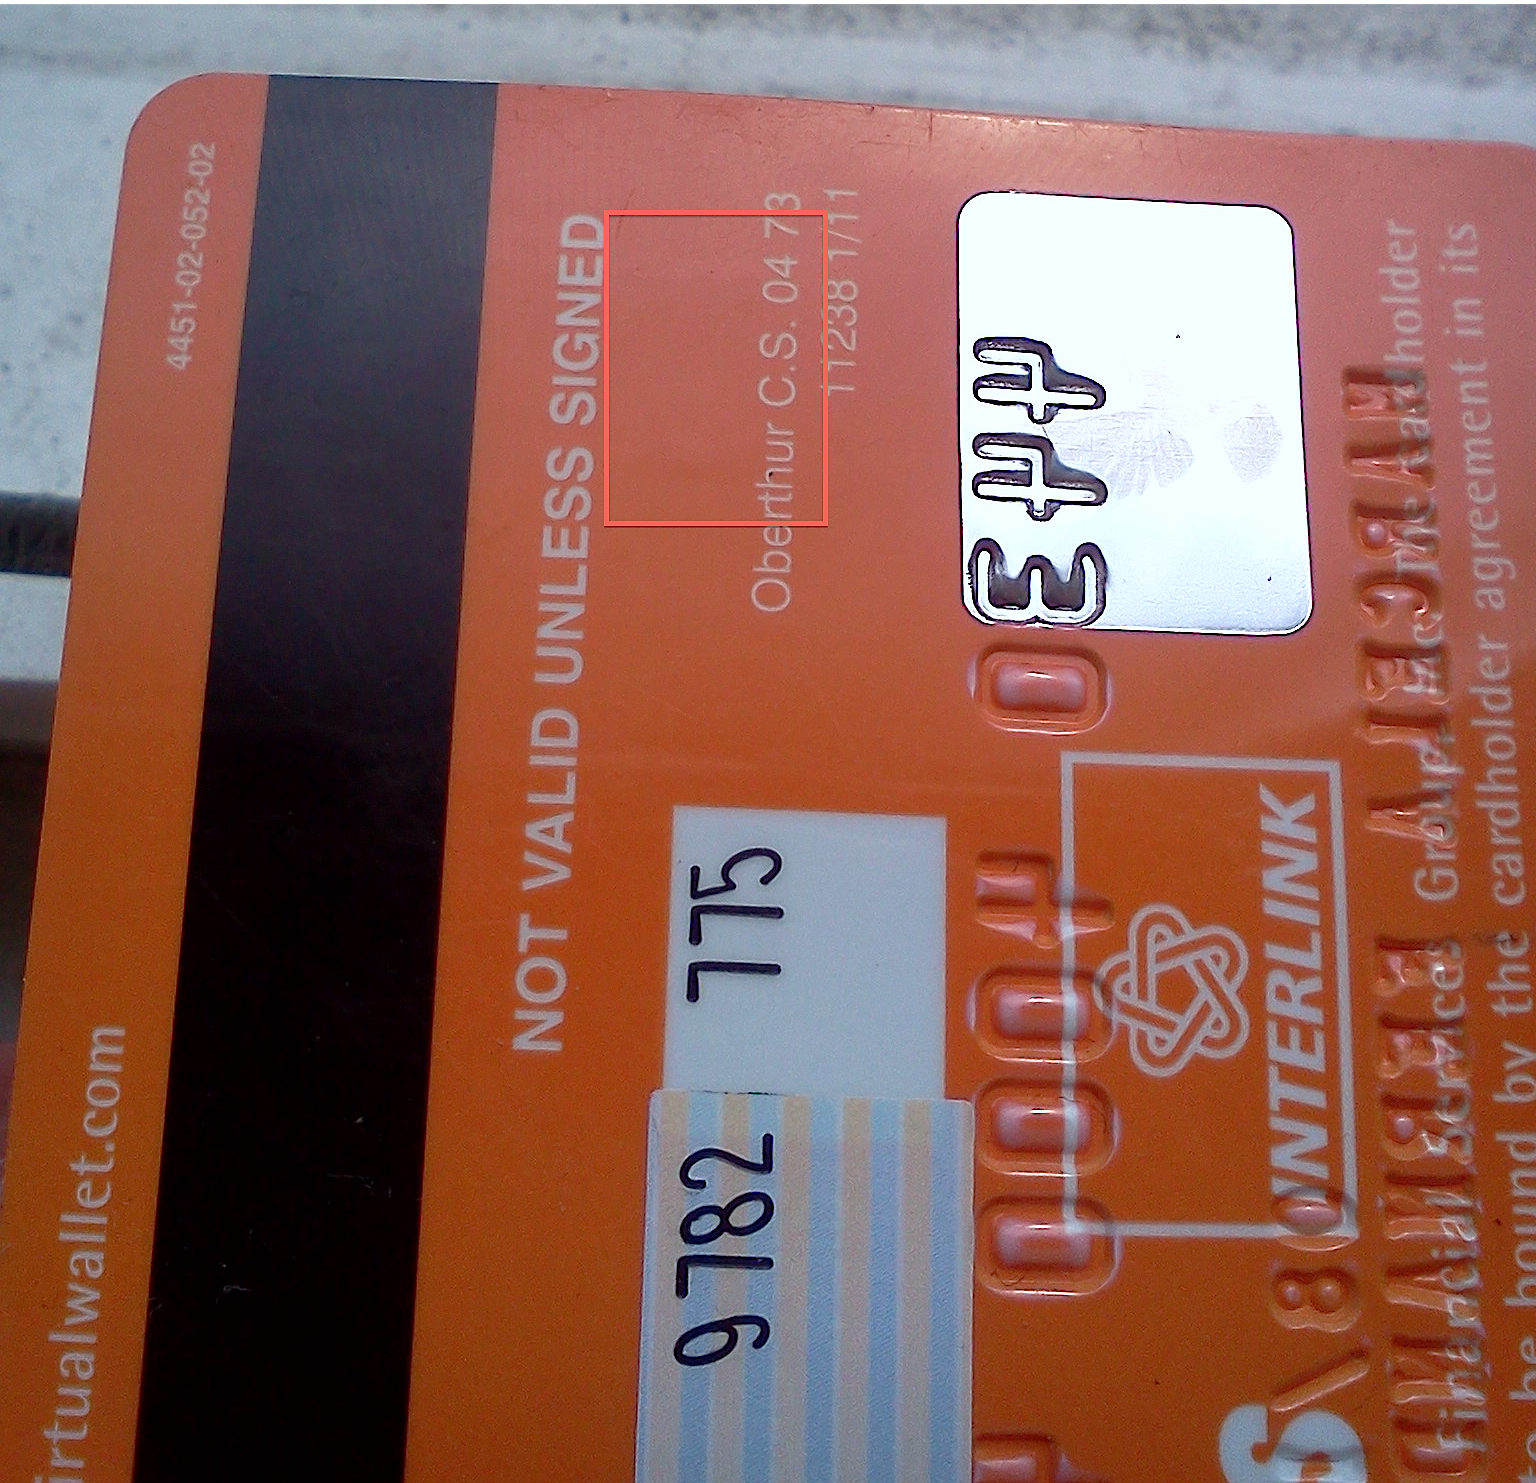
\includegraphics[width=0.3\textwidth]{images/RFID_in_PNC_Card.png}
	  \caption{Identifying an RFID chip}
	  \label{fig:RFID_in_PNC_Card}
	\end{figure}

	\begin{figure}%[H] %the [H] forces image placement
	  \centering
	  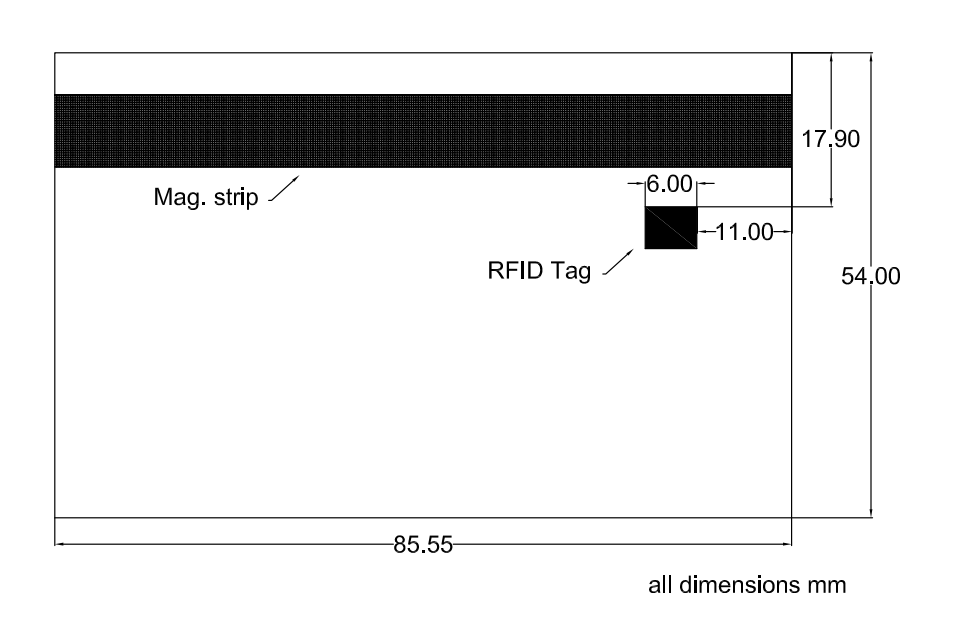
\includegraphics[width=0.4\textwidth]{images/RFID_chip_location.png}
	  \caption{Tag location: PNC payWave}
	  \label{fig:RFID_chip_location}
	\end{figure}

A warning for the user who would rather keep RFID tags intact: maintaining a safe 10 cm distance between RFID cards and devices is advisable, but as these objects naturally inhabit the same physical space, it would be unwise for a user to rely on this defense alone.  Assuming a user can continuously keep cards and readers separate, this defense only blocks a distributed attack from a phone that is physically in the user�s control; as discussed above, an attacker able to read a fully-functioning RFID card at close range will still be able to do so, and need only do so once to compromise the victim�s data.

Another word about distributed attacks: the same common sense caveats to Google Play application downloads apply even more so to the NFC-enabled user.  Be wary of the permissions an application requires.  If an application asks for more permissions than it needs, it could well be doing more than it says.  Google Play is still an unregulated market.  Consider downloading from a curated source.  The uninfected phone will not exfiltrate data.  

Each defense, regardless of its relative merits, postulates a level of user awareness of the inherent risks of RFID.  For a user to decide on the most suitable defensive measures for mobile pickpocketing, she must first be aware of the technology she possesses and its configuration.  Approximately 100 million RFID-enabled cards are currently in circulation \cite{forbes-1}.  Through the course of our research, it seems many users are unaware that these devices are already a part of their everyday lives.  An ignorant user is a less-wary user and an easier target for a mobile pickpocket.

\subsection{Long-term}
Current RFID credit and transit cards require no authentication and implement no encryption.  With no built-in defenses, mobile pickpockets who use applications to read sensitive information may not even qualify as hackers; they simply implement an open protocol \cite{bt-hacking-nfc-ccs}.  With payment and transit cards willing to divulge their data to any inquisitor with the correct sequence of commands, any consumer data stored on these RFID cards is at continual risk of exfiltration.  As consumer NFC technology is becoming more pervasive in mobile devices, that risk will only increase.

This level of exposure is surprising, considering that measures to secure RFID transactions of sensitive information are currently implemented in other domains.  Although RFID cards lack the power to perform the necessary functions for data security analogous to those seen in, say, TLS communications, some RFID cards do provide better than non-existent security.  E-Passports, for instance, implement a PKI, facilitating secure encryption, and they also link optical and RFID information, requiring information from both sources to access chip data, rendering the pickpocketing attacks described in this work moot \cite{security-privacy-epassports}.  The Navigo card used in Paris� mass transit system stores no personally identifiable information on a card; instead, each card has an id number \cite{bt-hacking-nfc-ccs}.  Using encryption, authentication, and digital signatures, a point-of-service terminal can take the information stored on the card and use it to access sensitive information from the company through a secure channel between the company and the point of service.  This system prevents users from carrying their data around with them, minimizing the damage from a pickpocketing attack.  By not aiming to secure NFC itself, choosing instead to focus on securing the service that implements an NFC transaction, sensitive data is better secured despite the limited resources of an RFID card.  

Perhaps U.S. credit card companies are getting wise to their card vulnerabilities.  As of January 2012, U.S. credit card companies are looking to not only further secure contactless cards, but ``...[move] toward a world beyond plastic...'' \cite{emv-upgrade}, better able to meet a variety of payment needs.  Looking forward, as mobile hardware moves toward widespread implementation in consumer mobile devices, working within the strict computational confines of RFID chips will be a far less attractive option. By comparison, industry and consumers alike will likely favor more robust device-based interactions over similar implementations using smart cards.  In this way, the mobile devices that make mobile pickpocketing such a dangerous problem are simultaneously the most attractive solution to the problem.     

The advantages of mobile devices over RFID cards are many.  With current technology, such devices already possess formidable computational power.  A typical smart phone has all the resources necessary to implement authentication, cryptography, and key management, allowing for functions like secure Internet browsing.  In Google Wallet, these functions are delegated to a so-called ``secure element,'' further cordoning off the application�s cryptographic functions.  As in any modern operating system, mobile devices ship with native security features as well, including encryption, password protection, certificate storage, and locking screens.  Combining these standard features with those implemented within an NFC payment application, such as Google Wallet \cite{google-wallet-security-1} provides for multiple layers of authentication before data access is granted.  This level of depth and variety in security features makes mobile application-based payment an easy choice over RFID cards.  

While these phones do have far greater security capabilities, it�s worth noting that mobile devices are not without security flaws of their own.  Google Wallet in particular has had several known problems \cite{google-wallet-pin-cracked} \cite{smartphonechamp-second-major-flaw-google-wallet}.  Such flaws can be expected; the technology is still maturing.  Undoubtedly, as such applications endure further analysis from the security community, security for NFC payment and transit applications will advance.  Better understanding current security shortcomings in NFC-enabled mobile devices will undoubtedly pave the way for future improvement.

Some important fixes to better secure users against mobile pickpocketing are possible now.  Application market management appears highly effective \cite{electronista-mcafee-malware-surge}.  While the open Android market provides the utmost in variety, its unfettered freedom provides fertile ground for the rapid growth of malware.  Some attribute Apple�s relative freedom from malicious iOS applications to its policy of strict capability limitations and application review.  Amazon recently opened a curated Android market \cite{amazon-android-appstore}; the impact of such curation on the security of Amazon-provided applications will be interesting to see.  

A regulated marketplace would do well to identify always-on applications, such as live wallpaper, that use NFC functionality.  Devices implementing NFC for no clear reason should be blocked.

\section{Future Work}
Time limitations of the semester prevented us from implementing a distributed attack.  Given the primary motivation for owning a mobile device is anytime, anywhere data connectivity, our efforts seemed better spent researching and implementing a physical attack:  after achieving that goal, simply sending captured data would likely prove a trivial feature to implement.  Now that we have developed card-reading capability, the next logical step would be to develop a seemingly benign application (likely a live wallpaper or game) and use that legitimate portion of the application as a front for reading and stealthily exfiltrating RFID information gathered by the device on which our application is installed.  

Sending data over NFC in Android is now easier still.  In Android version 4.0, Google has added Android Beam, \cite{ieee-beacon-mobileos-review} to its NFC library to facilitate peer-to-peer NFC communications.  While the Google API suggests Beam will help users ``share contracts, web pages, and videos with other devices,'' \cite{android-developers-beam} any further encouragement of NFC data transfer may also serve a mobile pickpocket.  Could a malicious program allow for piggybacking unauthorized, sensitive NFC data along with transmissions from legitimate applications?  An in-depth look at those possibilities and their facilitation through Android Beam would be an interesting progression from this research.       

We found no balance data stored on the Visa payWave card, but not so for the Clipper card.  As the Clipper is a Mifare DESFire card, with no known successful attacks \cite{farebot-1}, a next step in our research may involve implementing such an attack.  We have found the file where balance data is stored on the Clipper card.  As most of our team is moving to Silicon Valley where Carnegie Mellon has no fare agreements with municipal transportation comparable to those available to its students in Pittsburgh, arbitrarily increasing the available balance on the card would be an interesting attack.  What defenses are in place?  Along with the current balance updated with each fare interaction, the card�s files contain a card ID number.  Is the balance on the card associated with a balance record stored on the server-side?  What other fraud prevention measures are in place?  What measures could be implemented?  As most public transit systems are woefully underfunded, a widespread free-ride hack could be extremely damaging.

Some suggest that replacing the credit card number stored on the RFID tag with a different identification number assigned by the card companies. While this certainly thwarts a mobile pickpocket from collecting a credit card number, it still leaves the victim�s data compromised. An attacker could use an application such as ours to read this new ID from someone�s credit card and subsequently perform a replay attack by emulating the tag for fraudulent payments at any one of many NFC-enabled payment kiosks.  Adding the ability to store and replay such information would diversify the threats of a future mobile pickpocketing application.  

Recently, researchers from the University of Pittsburgh have discussed their work on a design to build a physical switch into RFID-enabled cards which would enable the RFID tag only when physically touched in a specific area. This is one promising solution to the contactless attacks described in our research. \cite{upitt-rfid-switch}

\section{Conclusion}
The primary takeaways from our research into mobile pickpocketing are as follows.  Despite any evidence or lack thereof of its occurrence in the wild, mobile pickpocketing is a legitimate threat to a user.  Users should be made aware of the technology and its risks, along with known defenses, so they can choose a course of action appropriate to their needs.  Given the current climate of NFC implementation, the longer the public is ignorant the more vulnerable it will become.

\section*{Acknowledgements}
We would like to thank a few gracious individuals, without whose help the success of this research would not have been possible.  First and foremost, we thank Dr. Patrick Tague who inspired the team inside and outside the classroom.  Thanks also to Theo Brower and Sushmita Subramanian for putting user data onto our Clipper card, knowing full well our malicious intents.  Thanks also to Andrew Santell who, after seeing our application, was immediately moved to destroy the RFID tag in his PNC payWave card, giving us first-hand evidence of an evidently viable mobile pickpocketing defense.  Thanks also to Marcela Fernandez, who donated a defunct PNC payWave card to help further our research.

%--REFERENCES--------------------
%\bibliographystyle{plainnat}
%\bibliographystyle{amsplain}
\bibliographystyle{acm}
\bibliography{adhawk-mobilepickpocketing}

\nocite{*}
%--------------------------------

\end{document}

